\chapter{Software Requirements \& Survey}
\label{ch:software_requirements}

In order to assess which technologies to use for a new project, one first has to take into account the kind of software product to build, the sector of the economy it will be used in as well as the specifics and constraints of the environment it's going to operate and interconnect in. Let us first take a closer look at those points:

\begin{itemize}
	\item \textbf{The kind of product} to construct will often determine some core technologies: Building a messenger app requires real-time behavior some statistical product suite would never make use of. Likewise, an autonomous control system of a space probe will also depend on time-critical components, but in a different way than a messenger app, relying strongly on a constant rate of throughput, whereas a message flow will not be critically disturbed by a lag or latency disruption every now and then.
	\item \textbf{The industry sector} largely determines requirements in the form of compliance or industry certification. For instance, whereas the security concerns in a normal end-user centered application might be dealt with with relatively moderate levels of effort, applications employed in the financial or even medical sectors will in all probability have to satisfy additional security demands such as audit trail systems or compliance to specific data formats and standards.
	\item \textbf{The technical environment} a system is operated in will influence its shape and behavior as well. A relatively disconnected and isolated system like a statistical module (which e.g. outputs some results on a nightly basis) will be modeled differently than a web-based, cloud-oriented service incorporating many interfaces and API calls to dependent background or partner services.
\end{itemize}

In the following sections, we are not considering the entire SW development workflow from an economic / managerial point of view, but just the technological aspects of it. Let us first realize the differences between software development today and the way it was usually conducted as short as only 2 decades ago.

The traditional software development process as followed throughout the first decades of the existence of our field has been relatively simple: upon setting a goal for functionality or any other measurable entity (code module, UI section), a continuous iterative process of writing some lines of code, re-compiling, testing (automated or manual) and bug fixing was all, or most, that was necessary to arrive at some usable product. Modern applications, however, especially web-based ones (and that includes all kinds of mobile apps that have seen their rise over last decade) operate on many different moving parts:

\begin{itemize}
	\item Some server-side backend which coordinates incoming requests and provides consistency across business logic and database layers. This is probably the part with the greatest similarity to traditional, client-only or centralized software (development). I would also include old-fashioned web 'applications' (and certainly websites) in this environment, as a browser-based GUI alone without much processing or business logic going on, does not really fall into the category of a distributed application.
	\item A client part in the form of a modern in-browser based app (like GMail, Google Docs or Office365) or any mobile app executing on a contemporary mobile device.
	\item Some background-services, mostly in separated modules distributed over one or many servers worldwide, including interfaces to dependent services, isolated REST services (like a search portal for medical professionals inside a larger healthcare application) or microservices: sub-components of the business logic implemented directly on a database level, as implemented in the Foxx application micro-framework inside the multi-model database ArangoDB \citep{Foxx2014}.
	\item Where needed, a visualization module will have to be provided which resides on the client side but is logically separated from the 'normal' business and communication logic of that module. In browsers, this can either be written in normal DOM code, SVG, Canvas, or WebGL (we don't want to mention earlier technologies that are fortunately falling from grace rapidly...).
\end{itemize}

In addition to this generic complexity, we have to deal with a different workflow cycle even on the level of individual developers: Whereas 15 years ago somebody could set up some HTML files, include some JavaScript files, iteratively add new snippets of code and check the results by reloading the browser, even this small part of the development cycle has changed dramatically over the past 10 years - new Meta-languages like Typescript or Coffeescript on the language side, HTML-meta-markups like HAML, CSS preprocessors like Sass/Scss/Less as well as the integration of modern testing libraries makes a simple browser reload a technique of the past.

Those new methods provide great opportunities (but also challenges) even for the single programmer, which require a whole execution and deployment infrastructure, as depicted in Figure~\ref{fig:webdev_cycle_components} and described in the following sections.

\begin{landscape}
\begin{figure}[ht]
	\centering
	\hspace*{-1cm}
	\vspace*{1cm}
	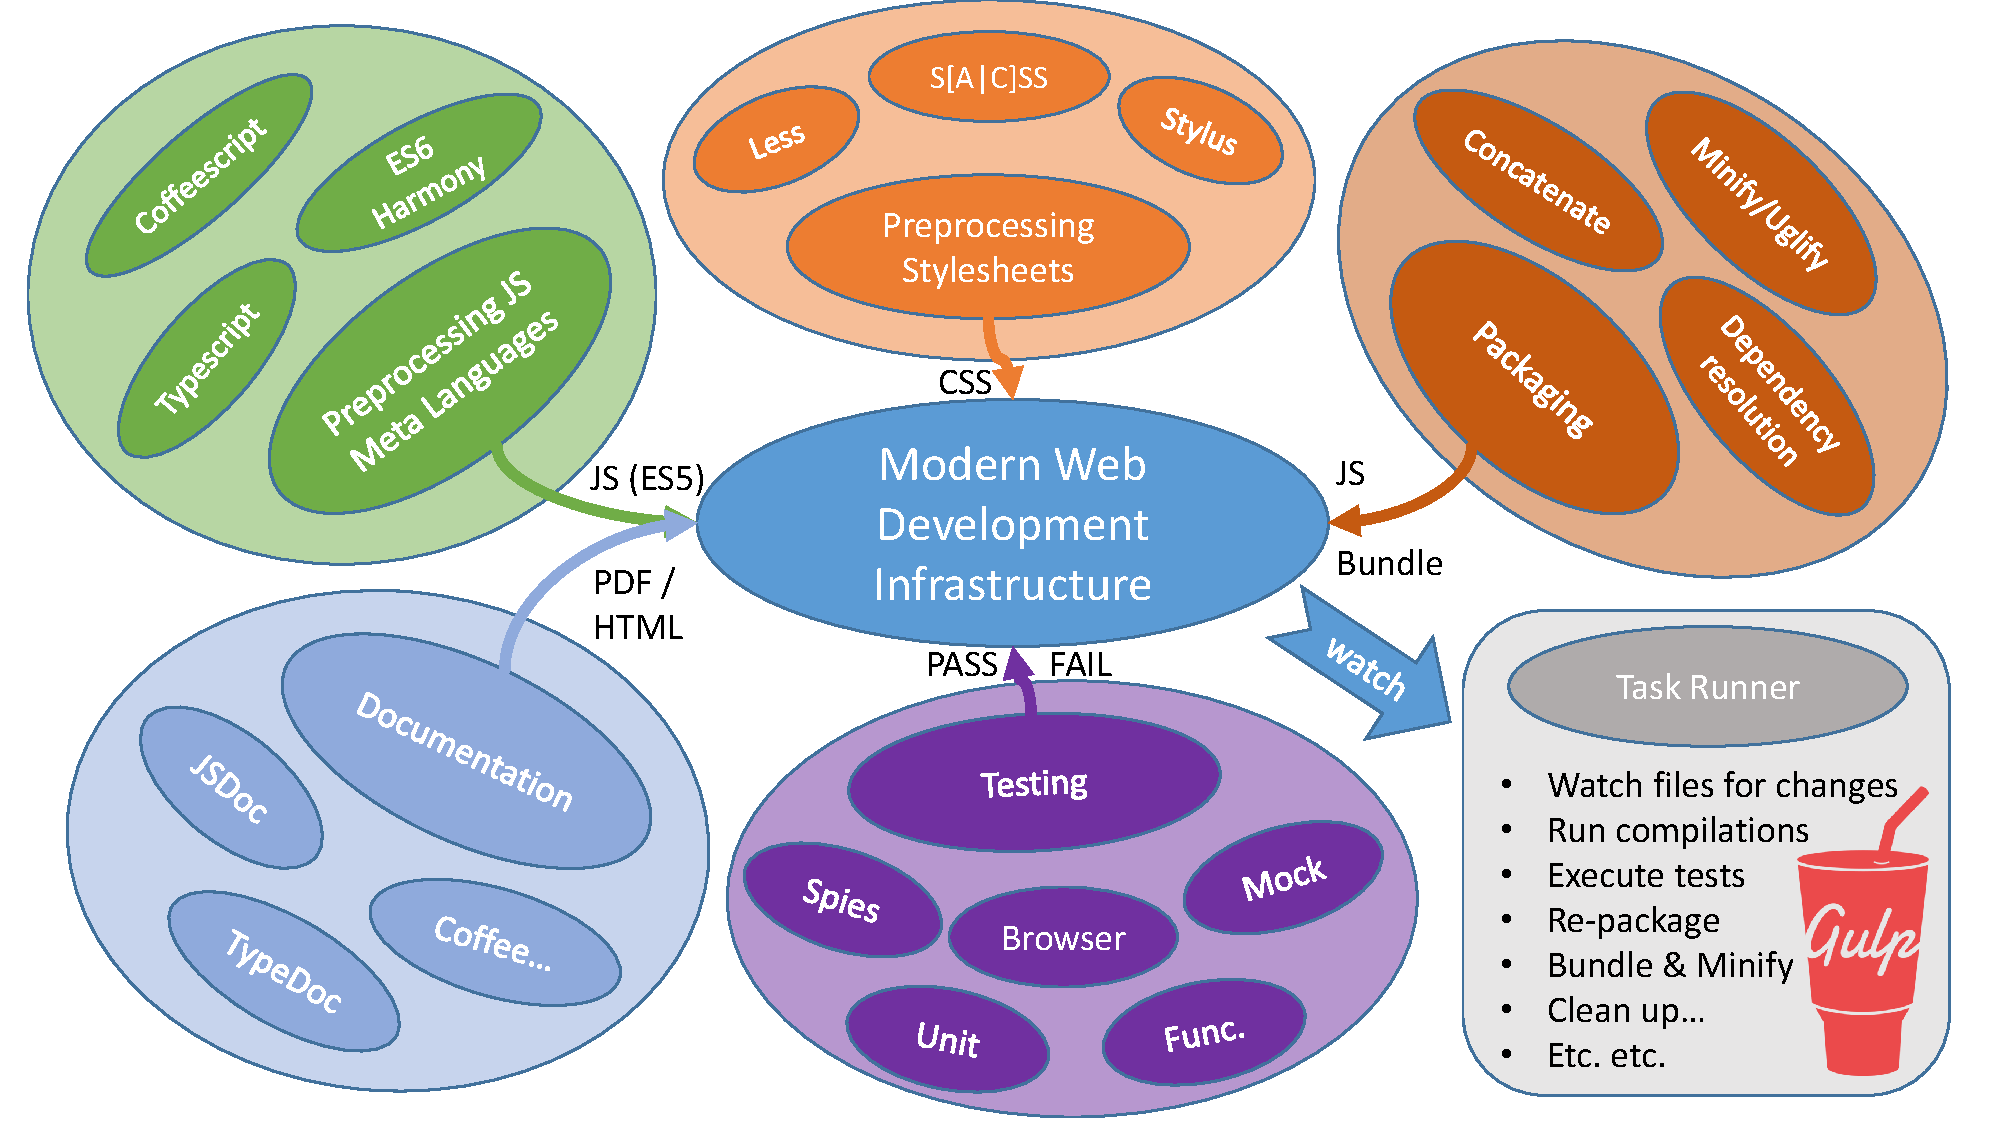
\includegraphics[width=1.8\textwidth]{figures/Modern_Web_Dev}
	\caption{Modern Web Development Component Diagram}
	\label{fig:webdev_cycle_components}
\end{figure}
\end{landscape}


\section{Preprocessing (compiling) JS Meta Languages}
\label{sect:language}

	\subsection{Javascript / ES6}
	\label{ssect:js_es6}
	
	Although the JavaScript language was put together by Brendan Eich of the Netscape company within 3 weeks in 1994 (when it was initially called LiveScript, and in 1995 renamed to JavaScript in a marketing attempt to jump on the Java-hype bandwagon), it turned out to be a nifty little language for general in-browser development and computations. JavaScript is a prototype based language, which means that it uses pointers to parent objects instead of class instantiations, features first-order functions (functions which can generate functions) and function-as-object passing, which is ideal for callback-based implementations of the visitor pattern, even more so as JS functions are automatically closures (functions or lambdas that have, regardless of their execution context, full access to their original definition scope).
	
	After almost two decades however, the JS development community felt that requirements on modern web-based products had increased so drastically that traditional JavaScript could only partially serve them anymore. Problems are, amongst others: 1) the lack of an explicit type system (which is crucial for larger software projects), 2) the lack of an internal module system allowing for requiring other files or packages (except in the form of browser script tags), 3) the lack of a chaining system for async callbacks (which resulted in the notorious 'pyramid of doom'), 4) the somewhat peculiar functional scoping, which is mostly an entrance barrier to developers of other languages, as well as 5) a general lack of elegant language constructs (like deconstruction of objects into variables etc.).
	
	While some of those problems have been addressed even in the context of ECMAScript 5 (like the introduction of promises to replace nested callback functions), many shortcomings could only be addressed by external libraries, which polluted the workflow with additional dependencies not needed in more sophisticated languages and often increased the JS download size by hundreds of kilobytes, which routinely becomes a problem on mobile devices.
	
	ECMAScript 6 (codename harmony) is an overhaul of the JavaScript language featuring classes, a new keyword for the familiar block scoping (\textit{let}), as well as an integrated module system allowing to require external files even inside the browser. The greatest obstacle to using ES6 today is the lack of complete support across all browser vendors - this is where ES6-to-ES5 compilers like \textit{Traceur} or the more popular \textit{Babel} come in. As far as syntax goes, ES 6 cleans up some keyword usages in order to make code more readable.	
	
	\begin{lstlisting}[caption={ECMAScript 5 (usually referred to as 'JavaScript') version of functional programming using the natively built-in mapping function.}, label={fig:ECMAScript5_mapping}, language=JavaScript]
odds  = evens.map(function (v) { return v + 1; });
pairs = evens.map(function (v) { return { even: v, odd: v + 1 }; });
nums  = evens.map(function (v, i) { return v + i; });
	\end{lstlisting}	
	
	\begin{lstlisting}[caption={ECMAScript 6 equivalent to the above code.}, label={fig:ECMAScript6_mapping}, language=JavaScript]
odds  = evens.map(v => v + 1)
pairs = evens.map(v => ({ even: v, odd: v + 1 }))
nums  = evens.map((v, i) => v + i)
	\end{lstlisting}
	(Examples taken from \citep{ES6Features})
	
	Although ES6 is a great improvement over ES5 in many respects, it still lacks an explicit type system and interfaces (which can guide an IDE in it's analysis regarding Code Completion and IntelliSense). It was therefore not considered the best option for the development of a potentially large library as GraphiniusJS.			
	
	\subsection{Coffeescript (CS)}
	\label{ssect:coffeescript}
	
	Coffeescript was an attempt to make JavaScript code more readable as well as writable. It was apparently inspired by the clean syntax used in modern scripting languages like Ruby or Python and adopted the use of whitespace as control characters like Python (but not Ruby). Most of the language was based on using 'syntactic sugar' to abbreviate otherwise verbose JS code. For instance, the  \textit{this} variable was replaced by the  \textit{@} sign, the return statement at the end of a function became superfluous, and the lambda operator \textit{->} was introduced as a shortcut for the \textit{function} keyword in normal JS.
	
	\begin{lstlisting}[caption={Two versions of the same mapping functionality in CoffeeScript}, label={fig:Coffeescript_mapping}, language=JavaScript]
[1..10].map (i) -> i*2
i * 2 for i in [1..10]
	\end{lstlisting}
	\small
	(Example taken from \url{CoffeeScript})
	
	Like ES6, Coffeescript is compiled down to ES5 through it's own coffee compiler. As much as the idea of CS is neat and very justified for individual developers, the use of whitespace as control characters can add some additional hassles if working in a team; only slight deviations in the individual setup can cause serious problems, like the use of editors that use different representations for tabs (tab vs. 2 spaces vs. 4 spaces) or different line ending symbols (Windows vs. Mac vs. Linux). Furthermore, CS did not resolve the lack of an internal module system or the lack of an explicit type system, and was therefore not considered for Graphinius JS.
	
	
	\subsection{Typescript (TS)}
	\label{ssect:typescript}
	
	The greatest obstacle to large-scale web-development in ES5 was the lack of an explicit type system and built-in module system, which would allow an IDE to scan dependent files and constructs and infer a valid type-flow, enabling the development environment to assist the programmer with code completion and type error hints. This was realized by Microsoft when they ported part of their Office suite to the web (Office365), which consumed not only years of manpower but took hundreds of thousands of lines of code before a stable product could be released. As a consequence, they formed a group around their lead C\# / .NET developer Anders Hejlsberg (the former creator of TurboPascal and chief software engineer at Borland until 1996) with the mission to develop a JS meta language incorporating those characteristics for large scale web development in 2012. The result of those efforts is Typescript, which of 2016 is a superset of ES6 with the additional benefits of allowing for the declaration of interfaces, enums, and in-place type annotations (amongst many others features like default and optional function parameters): 
	
	\begin{lstlisting}[caption={Typescript sample featuring import of an external module, an exported interface definition, type annotations, instance variable setting via constructor specifiers (protected) as well as optional parameters}, label={fig:TS example}, language=JavaScript]
import * as $N from "./Nodes";

export interface IConnectedNodes {
	a: $N.IBaseNode;
	b: $N.IBaseNode;
}

class BaseEdge implements IBaseEdge {
	protected _directed		: boolean;
	protected _weighted 	: boolean;
	protected _weight		: number;
	protected _label		: string;
	
	constructor (protected _id,
		protected _node_a:$N.IBaseNode,
		protected _node_b:$N.IBaseNode,
		options?: EdgeConstructorOptions) {...}
}	
	\end{lstlisting}
	\vspace{-0.3cm}
	\begin{center}
		\small
		(Example taken from the Graphinius JS Edge Class)
	\end{center}
	
	Furthermore, the Typescript compiler can output TS code to ES6, ES5 or even ES3, and already incorporates some features currently only found in the ES7 draft specification (which will take several years to become the next standard). With all the benefits offered by ES6, no additional compile step (over ES6 with traceur/babel) and additional typings support (which comes in the form of separate typing files that even exist for most external libraries like underscore, lodash or jquery), Typescript made an ideal candidate as the base language for Graphinius JS.
	

\section{CSS preprocessing}
\label{sect:css_preproc}

	Just like the requirements on JavaScript underwent a steady evolution as project sizes went from very small-scale Webpages to full-blown in-browser application suites, so did the demands on Cascading Style Sheets (CSS) increase over time. The original CSS specification did not offer any possibilities of abstraction or code-reuse, for example. There were no modules that could be included and shared, no parameters one could pass to instructions (like the pixel width a border-radius should exhibit) nor any variables one could set as defaults (for the purpose of color-scheme definitions, for instance). Several projects have sprung up in order to amend that situation. Let's briefly take a look at 2 options, namely SCSS (SASS, which is just SCSS without braces and semicolons) and LESS, which runs the pre-processing step on the client rather than the server:
	
	\begin{lstlisting}[caption={SCSS example demonstrating the use of variables and mixings}, label={fig:scss_preproc}, language=CSS]
$font-stack:    Helvetica, sans-serif;
$primary-color: #333;
@mixin border-radius($radius) {
	-webkit-border-radius: $radius;
	-moz-border-radius: $radius;
	-ms-border-radius: $radius;
	border-radius: $radius;
}
body {
	font: 100% $font-stack;
	color: $primary-color;
}	
.box { @include border-radius(10px); }
	\end{lstlisting}
	\small
	(Example taken from \citep{SassBasics})
	
	
	\begin{lstlisting}[caption={LESS example demonstrating the use of variables and default parameters}, label={fig:less_preproc}, language=CSS]
@base: #f938ab;	
.box-shadow(@style, @c) when (iscolor(@c)) {
-webkit-box-shadow: @style @c;
	box-shadow:         @style @c;
}
.box-shadow(@style, @alpha: 50\%) when (isnumber(@alpha)) {
		.box-shadow(@style, rgba(0, 0, 0, @alpha));
}
	\end{lstlisting}
	\small
	(Example taken from \citep{LessCSS})
	
	While CSS preprocessors are important in every contemporary web project, the work described in this Master Thesis is focused on the underlying graph library, which features no (built-in) graphical component and therefore did not require any such module.
	
	
\section{Testing}
\label{sect:testing}

	With the increase in size and complexity of JavaScript codebases, testing became essential in the modern web development cycle. While there are several other JS (unit) test frameworks available (like JSUnit, QUnit, YUI-Test), we will mention only two contemporary libraries in detail, which both allow for behavior driven development (BDD) style testing as well as \textit{mocking}, \textit{stubbing}, and \textit{spying}. Both have very similar syntax and are intermixable with different assertion libraries; it seems to the author that a choice between those libraries is more a question of taste than necessity, and for GraphiniusJS, a combination of Mocha with Chai has been chosen.

	\subsection{Jasmine}
	\label{ssect:jasmine}
	
	Jasmine \citep{hahn2013javascript} is modeled after the Ruby RSpec Gem and refers to its tests as \textit{specs}. It allows for nesting of \textit{describe} blocks in order to distinguish different levels of test suites, follows the \textit{should} approach by providing \textit{it} functions taking a description of a test as well as it's test body in the form of a callback. An assertion library is built right into Jasmine and uses the \textit{expect} style of writing assertions. Let's have a look at a small example:
	
	\begin{lstlisting}[caption={Jasmine example of a nested test suite containing one simple assertion in expect style as well as a spy and a stub}, label={fig:jasmine_expect}, language=JavaScript]
describe('calculator', function() {
	describe('add()', function() {
		it('should add 2 numbers togoether', function() {
			expect(calculator.add(1, 4)).toEqual(5);
		});
	});
});
// now for spying...
var userSaveSpy = spyOn(User.prototype, 'save');
// and stubbing...
spyOn(user, 'isValid').andReturns(true);
	\end{lstlisting}
	\small
	(Example taken from \citep{JSTestTest})
	
	
	\subsection{Mocha / Chai}
	\label{ssect:mocha_chai}
	
	The Mocha test runner basically provides the same functionality as Jasmine in that it provides \textit{describe} blocks, should-style \textit{it} functions and several ways to output reports (spec-style, list, dots, the nyan cat...) as well as handle pending tests (via not handing a callback to the \textit{it} function) or skipping tests (via \textit{it.skip();}). The greatest difference to Jasmine is the fact that Mocha does not ship with a built-in assertion library. There are several compatible alternatives, like \textit{should.js}, \textit{expect.js} or \textit{unexpected}. The most popular and widely used, however, clearly seems to be \textit{Chai}, which provides the \textit{should}, \textit{assert} as well as \textit{expect} styles of writing assertions. In addition to that, we also need a library called sinon.js that allows for spying and stubbing. We will be seeing some in-depth examples of Mocha, Chai (expect style) and Sinon in the Chapter~\ref{ch:implementation}, so let's limit ourselves to the same use case as above:
	
	\begin{lstlisting}[caption={Mocha example of a nested test suite containing one simple assertion in expect style as well as a spy and a stub}, label={fig:mocha_chai_sinon}, language=JavaScript]
describe('calculator', function() {
	describe('add()', function() {
		it('should add 2 numbers togoether', function() {
			// expect style
			expect(calculator.add(1, 4)).to.equal(5);
			// should style
			calculator.add(1, 4).should.equal(5);
			// assert style
			assert.equal(calculator.add(1, 4), 5);
		});
	});
});
// now for spying...
sinon.spy(user, 'isValid');
// and stubbing...
sinon.stub(user, 'isValid').returns(true);
	\end{lstlisting}
	\small
	(Example taken from \citep{JSTestTest})

	\subsection{Cucumber}
	\label{ssect:selenium}
	
	Cucumber describes itself as 'An open-source tool for executable specifications', which means it wants to be understood less as a testing tool but rather as a group communication tool. The idea behind cucumber is the 'single source of truth' concept, which means that both the specifications handed down to the developers by their customers or management as well as the technical test definitions that execute test suites and determine the project's progress from the programmers' viewpoint, should be one and the same document.
	
	The first and foremost implication of this approach is that the specifications must be formulated in plain English (or any other common-language), so that collaborators from outside the immediate project team can read, but ideally also write and modify them. It is then the job of developers to transfer those common-language statements via so-called \textit{step definitions} into executable test code. In invoking this test code, the cucumber test runner receives feedback on the internal state of test case completion, which is translated back up to the semantic common-language level and displayed as progress of the original specification. This way, both programmers as well as customers / managers can monitor the progress of the project, and tests become both functional as well as acceptance tests (with unit tests usually not being expressed via cucumber).
	
	A cucumber feature file is written using the so-called Gherkin syntax (a business readable, domain specific language) consisting of Feature and Scenario definitions. Features are general statements of intent describing the business value of a certain feature from the perspective of a potential user. Scenarios then describe different aspects of that feature in the form of usage scenarios the user might find herself in.
	
	\begin{lstlisting}[caption={Cucumber example describing a Feature containing a simple Scenario}, label={fig:cucumber}, language=JavaScript]
	
	Feature: Example feature
		As a user of Cucumber.js
		I want to have documentation on Cucumber
		So that I can concentrate on building awesome applications
		
		Scenario: Reading documentation
			Given I am on the Cucumber.js GitHub repository
			When I go to the README file
			Then I should see "Usage" as the page title	
	\end{lstlisting}
	
	The step definition file implementing the first of the three lines in the scenario could be implemented as follows:
	
	\begin{lstlisting}[caption={Cucumber example describing a Feature containing a simple Scenario}, label={fig:cucumber}, language=JavaScript]	
module.exports = function () {
	this.Given(/^I am on the Cucumber.js GitHub repository$/, function (callback) {
		this.visit('https://github.com/cucumber/cucumber-js', callback);
	});
};
	\end{lstlisting}
	\small
	(Examples taken from \citep{CucumberJS})
	
	Cucumber can be utilized from many different languages and has been used by the author as far back as 2009. In the case of Graphinius it will certainly be used once the platform module (browser UI) begins to take shape, as cucumber is very well suited to be used in combination with the browser DOM. For the scope of the underlying Graphinius JS library however, there was no reason to employ such a tool as collaboration with end-users on that level seems neither necessary nor sensible.


\section{Automatic Documentation}
\label{sect:documentation}

	Writing manual documentation on a software library is absolutely necessary if one desires their product to be used by other developers; writing documentation files separately from one's code files however is a burden not many programmers want to accept. This is were automated documentation generators come in - they scan the source code of a project for comments above a function or class definition and auto-generate the required documents in a convenient output format like HTML or PDF. 
	
	
	\subsection{JSDoc \& alternatives}
	\label{ssect:jsdoc}
	
	In the realm of JavaScript there are several candidates for pure, JS-based auto-doc generation; in a review conducted by \citep{JSDocRef}, the four libraries JSDoc, DOCCO, doxx and ui were examined for several properties, the most important of which were:
	
	\begin{itemize}
		\item Does it support structured syntax (like Javadoc)?
		\item Can the appearance be customized (via CSS or CSS frameworks like Bootstrap)?
		\item Does the output contain a search feature?
		\item Does it parse the entire source code or only the comment blocks?
	\end{itemize}
	
	The interested reader may be referred to the resource mentioned above; as we are using Typescript for Graphinius JS, we do not want to limit ourselves to capturing just the information present in the output JS, but also the type information as well as interface specifications only found in the original TS sources.
	
	\subsection{TypeDoc}
	\label{ssect:typedoc}
	
	Currently, there is only one library available for automatically scanning through Typescript sources and generating an appropriate documentation - TypeDoc. It extracts all type annotations found in interfaces or method specifications and scans Javadoc-like comment blocks. Its output is HTML5 with a convenient search function and customizable appearance as well as a practical legend for different types of entities (class, interface, function etc.); as of yet, it neither supports simple double-slash comments nor output to PDF. 
	
	A very nice feature to mention comes to bear in combination with a github project - in this case Typedoc is capable of directly linking an item's documentation to the appropriate place in the github repository, which makes switching from documentation to code a convenient experience. As the whole documentation for Graphinius JS exists in the form of extracted Typedoc and is readily available to the reader in Appendix~\ref{App:AppendixB}, we can forgo the display of a sample at this point.
	

\section{Build system for browsers / packaging}
\label{sect:build_browser}

	Within the server-side JavaScript version of NodeJS (which uses Google's V8 under the hood), one can easily require other files as modules through the CommonJS module specification. This of course is a superior way of building JS applications, as modules are thereby testable in isolation, dependencies can be required without adding some script tag into an HTML file, and dependency resolution is done via the built-in module framework as opposed to having to take care of including script tags in the right order (or otherwise they might overwrite each others' variables within the global namespace, which is a frequent source of attrition amongst web developers).
	
	Unfortunately, there is no native way to require JavaScript files or parts thereof from another JS file in the browser. With the advent of ECMAScript 6 this shortcoming will finally be corrected; however due to the fact that most browsers do not fully support that standard yet, and given the benefits of a 'normal' SW-development process, it has become commonplace to develop one's webapp in NodeJS (including all necessary libraries from the Node Package Manager's repositories), and then utilizing an external tool to package the software for its final release. Those tools have then to collect all the source files including dependencies, resolve any potential conflicts in the dependency graph, wrap each file's content with a require mechanism that works in the browser, and finally concatenate (and maybe minify / uglify) the result in order to save space.

	Although there are a few more candidates (RequireJS, SystemJS, JSPM) that could be mentioned in this section, we are only going to take a look at two libraries which characterize the differences in this field pretty well:
	
	
	\subsection{Browserify}
	\label{ssect:browserify}
	
	Browserify is easily the most popular amongst the various packaging libraries available, and probably also the most powerful in its ability of dependency checking and conflict resolution. Throughout the first months of developing GraphiniusJS, the author used browserify to conveniently package all of the code files into a bundle readable by the browser. The library is especially handy since it can deal with NodeJS specific dependencies like the Filesystem module, which provide no additional use in the browser but can be hard to extract out manually from the packaging process. In addition it resolves circular dependencies on its own, which is especially practical for less experienced programmers. The great disadvantage or browserify is the file size of its output: in order to offer all the benefits it provides, it generates in excess of 30k lines of boilerplate code for even the tiniest of JavaScript programs. This results in a file size easily in excess of 1MB, which renders browserify practically unusable for mobile applications.
	
	\subsection{Webpack}
	\label{ssect:webpack}

	Webpack, in many respects, is the opposite of Browserify. It does not offer a no-hassle, work-the-first-time experience for today's stressed web developer, requires some (often much) configuration of loaders for different file types, easily capitulates in the event of circular dependencies (and does not even fire an error or warning) and has serious problems including all kinds of NodeJS (server-side) libraries. Despite the greater configuration effort and necessary developer's care however, Webpack's require wrapper around JavaScript files and functions is microscopic compared to browserify. This way, the author was capable of packaging all of Graphinius JS (as of this writing) into 67.8 kilobytes of uncompressed and 25 kilobytes of minified JavaScript, with further down-potential in using a better compression library like Google's Closure compiler in the future (which requires its own delicate handling...).
	

\section{Task Runner}
\label{sect:build_system}

	Finally, all of the above components have to work in perfect coordination in order to make the web development experience convenient and leave the programmer to their most important job: focusing on the problems to solve rather than manually operating different libraries in the various preparation steps. Therefore, task runners (the JavaScript vocabulary's version of Makefiles) have been invented, which offer several standard tasks to be executed and countless more to be added via their respective plugin systems. The main duty of a task runner is to watch local files for changes (happening every time they are saved to disk) and execute different, predetermined tasks in a given order. In the context of Graphinius JS, this development cycle consisted of the following phases (only 1 and 2 are executed on every save, the rest required a separate 'make' call):
	
	\begin{enumerate}
		\item \textbf{Build:} Compile TypeScript to JavaScript.
		\item \textbf{Test:} Run all synchronous Mocha tests; for performance reasons, a few asynchronous tests like remote JSON graph structure loading were not periodically executed.
		\item \textbf{Generate Typedoc} and output the resulting HTML to a subfolder.
		\item \textbf{Assemble JS output} files and write them to the dist directory for requiring from a NodeJS console.
		\item \textbf{Package \& bundle (compress)} the dist folder's content using webpack and output a minified JavaScript file consumable by any standard web browser.
	\end{enumerate}
	
	In addition to those standard tasks, a library called \textit{Istanbul} was used to capture the progressing test coverage.


	\subsection{Grunt}
	\label{ssect:grunt}
	
	The	Grunt JS task runner has been around since early 2012 and follows the principle of \textit{Configuration over code}. This means that instead of writing executable code, the library takes a configuration file in the form of a \textit{Gruntfile.js}. Although this file is of generic JavaScript format, no real computations or control flows take place inside it; instead, Grunt takes instructions in the form of JSON object blocks, which makes writing a Gruntfile easy and intuitive, but severely limits the developer's possibilities to fine-tune desired functionalities.
	
	\subsection{Gulp}
	\label{ssect:gulp}
	
	Gulp JS, as a slightly more recent contender (the first commit logged on github stems from July 2013) represents the opposite approach to Grunt JS - it is based on the idea of \textit{Code over configuration}. This implies that instead of writing an extensive configuration file, a \textit{Gulpfile.js} is written like a normal JavaScript program, making extensive use of the NodeJS-native streaming capabilities to pass results of an earlier processing step on to a later (much like the Unix kernel pipes can be used). This gives developers greater power over their build process, enabling them to use normal language constructs like branches and conditional assignments.		
	
	\begin{figure}[ht]
		\centering
		\hspace*{-1.1cm}
		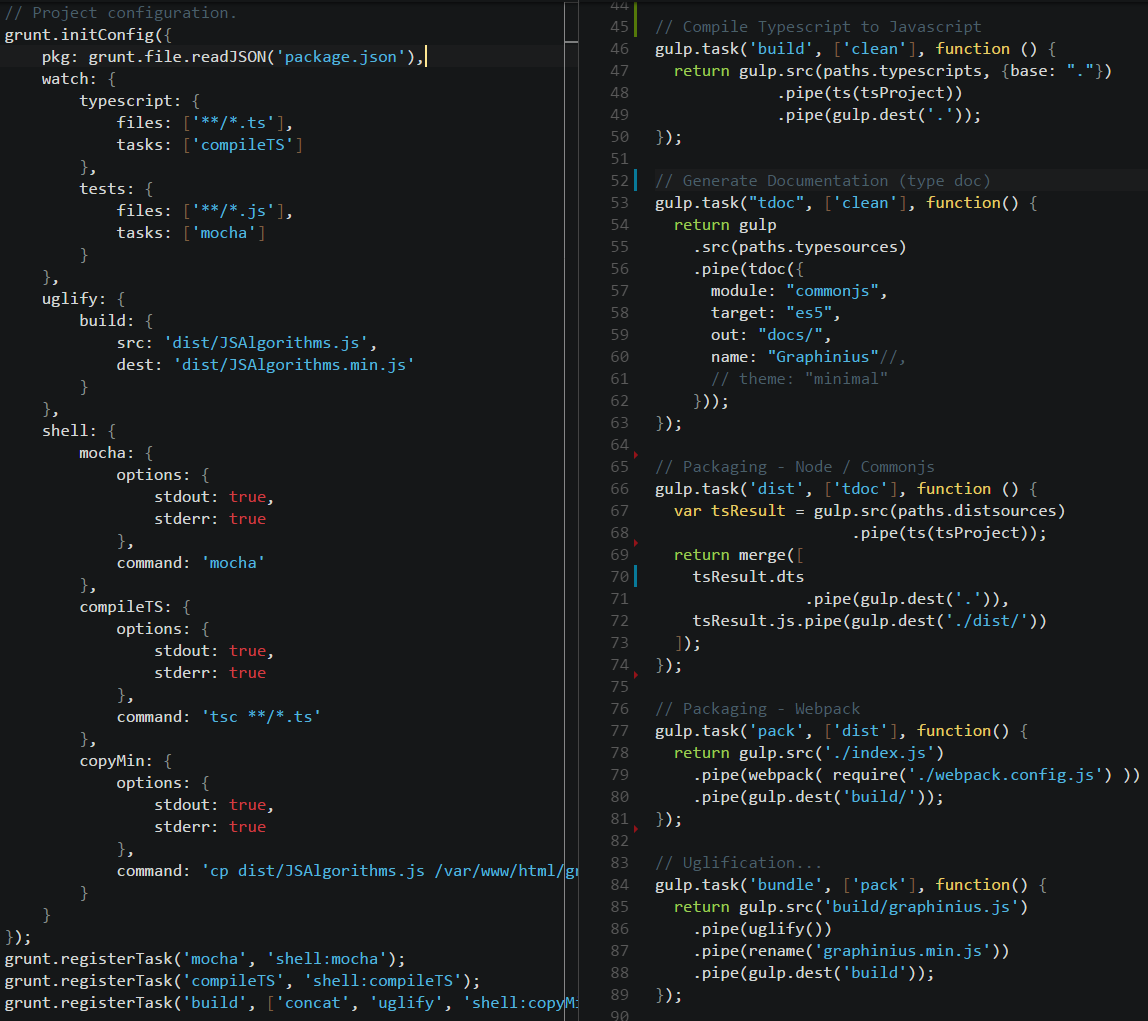
\includegraphics[width=1.15\textwidth]{figures/grunt_gulp_comparison}
		\caption{Comparison between Grunt \& Gulp build systems}
		\label{fig:grunt_gulp}
	\end{figure}
	

\section{Overview of technology choices}
\label{sect:design_choices}

In summary, the chosen technologies / libraries for developing Graphinius JS came to be:

\begin{itemize}
	\item \textbf{JS Preprocessor:} Typescript
	\item \textbf{CSS Preprocessor:} N/A
	\item \textbf{Testing libraries:} Mocha + Chai (expect style) + Sinon
	\item \textbf{Doc generator:} Typedoc
	\item \textbf{Packaging:} Webpack
	\item \textbf{Task Runner:} Gulp
\end{itemize}
